\section{GUI}

Single-Threaded (sonst hohes Deadlock-Risiko), nur UI-Thread manipuliert GUI (sonst Race Condition Risiko) \textcolor{red}{langlaufende/blockierende Operationen}, \textcolor{red}{von Worker Thread lesen/schreiben auf GUI}

\subsection{UI Dispatching - Java}
delegiert Komponentenzugriffe an UI Thread, UI Operation wird als Events in die UI Event Queue eingereiht

\textbf{verhindert Blockierung UI Thread}
\begin{lstlisting}
button.addActionListener(event -> {
  new Thread(() -> { // bis hier ist UI Thread (vorher von UI lesen!)
    var text = readHugeFile();
    SwingUtilities.invokeLater(() -> { // asynchron, bis hier ist Worker Thread
      textArea.setText(text); }); // wieder UI Thread versetzt
  }).start(); }); // UI Thread
\end{lstlisting}

\lstinline{invokeAndWait()} blockiert! erlaubt sequenzielle Auflistung in Worker Thread
%\begin{lstlisting}
%// Background Worker Beispiel -- notwendig?
%class BackgrCalc extends SwingWorker<Integer, Void> { // Int: Resultat von Background, Void: Zwischenresultat
%  @Override
%  public Integer doInBackground () { // separater Thread (zeitaufwendige Operationen als Task in Thread Pool)
%    return longComputation (); }
%  @Override
%  protected void done() { // UI Thread (UI-Zugriffe durch EventDispatchThread)
%    try { int result = get(); // gibt Resultat von doInBackground()
%      label.setText("Result: " + result); // UI Thread
%    } catch (InterruptedException|ExecutionException e) {
%    } } }
%\end{lstlisting}

\textbf{garantiert sequenzielle Reihenfolge} der Downloads und GUI-Operationen
\begin{lstlisting}
void download(List<URL> links, OutputStream output) {
    if (links.isEmpty()) { statusLabel.setText("All done!"); }
    var url = links.get(0);
    statusLabel.setText("Downloading " + url);
    if (cancelBox.isSelected()) { statusLabel.setText("Cancelled!"); return; }
    CompletableFuture.runAsync(() -> {
        url.openStream().transferTo(output); }
        var remaining = links.subList(1, links.size());
        SwingUtilities.invokeLater(() -> download(remaining, output)); }); }
\end{lstlisting}

\subsection{UI Dispatching - .NET}

\begin{lstlisting}
public class MainWindow : Window {
  private void startCalculationButton_Click(...) {
  calculationResultLabel.Content = "(computing)";
  int number;
  if (int.TryParse(numberTextBox.Text, out number)) {
    Task.Run(() => { // UI Thread ruft auf
    	int result = LongCalculation(number); // in anderen Thread outsourcen
    	Dispatcher.InvokeAsync(() => { // UI Update wieder als UI Event dispatchen
    	  resultLabel.Content = result; }); }); } } }

control.BeginInvoke(delegate) // WinForm
// synchron mit Invoke (ohne async)
\end{lstlisting}

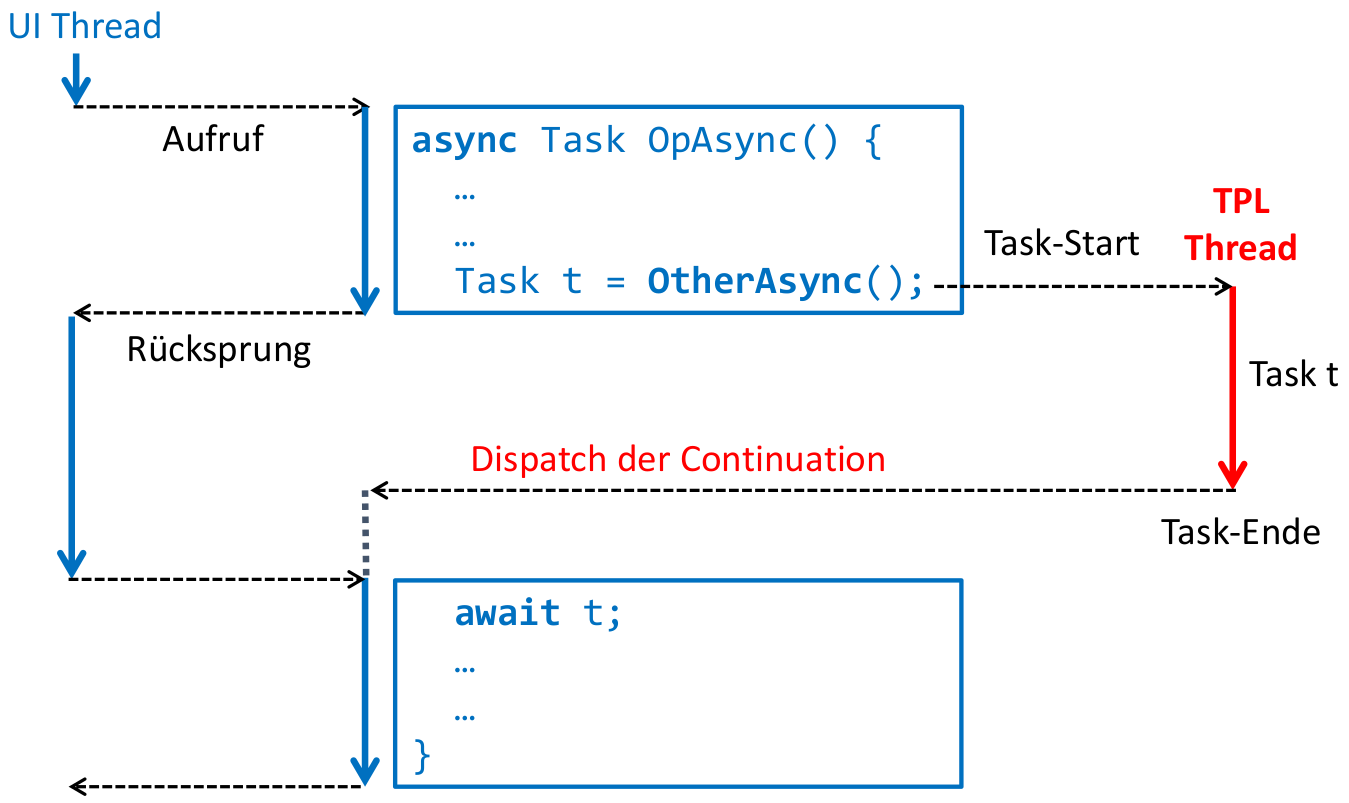
\includegraphics[width=0.7\linewidth]{03_ausfuerung-ui-thread.png}

wird als Event von UI-Thread ausgeführt


\textbf{async Function} \textcolor{red}{muss await enthalten} sonst Compiler-Warnung/keine Asynchronität \textcolor{red}{keine ref-/out-Parameter} Rückgabetypen \lstinline{void} \lstinline{Task} \lstinline{Task<T>}

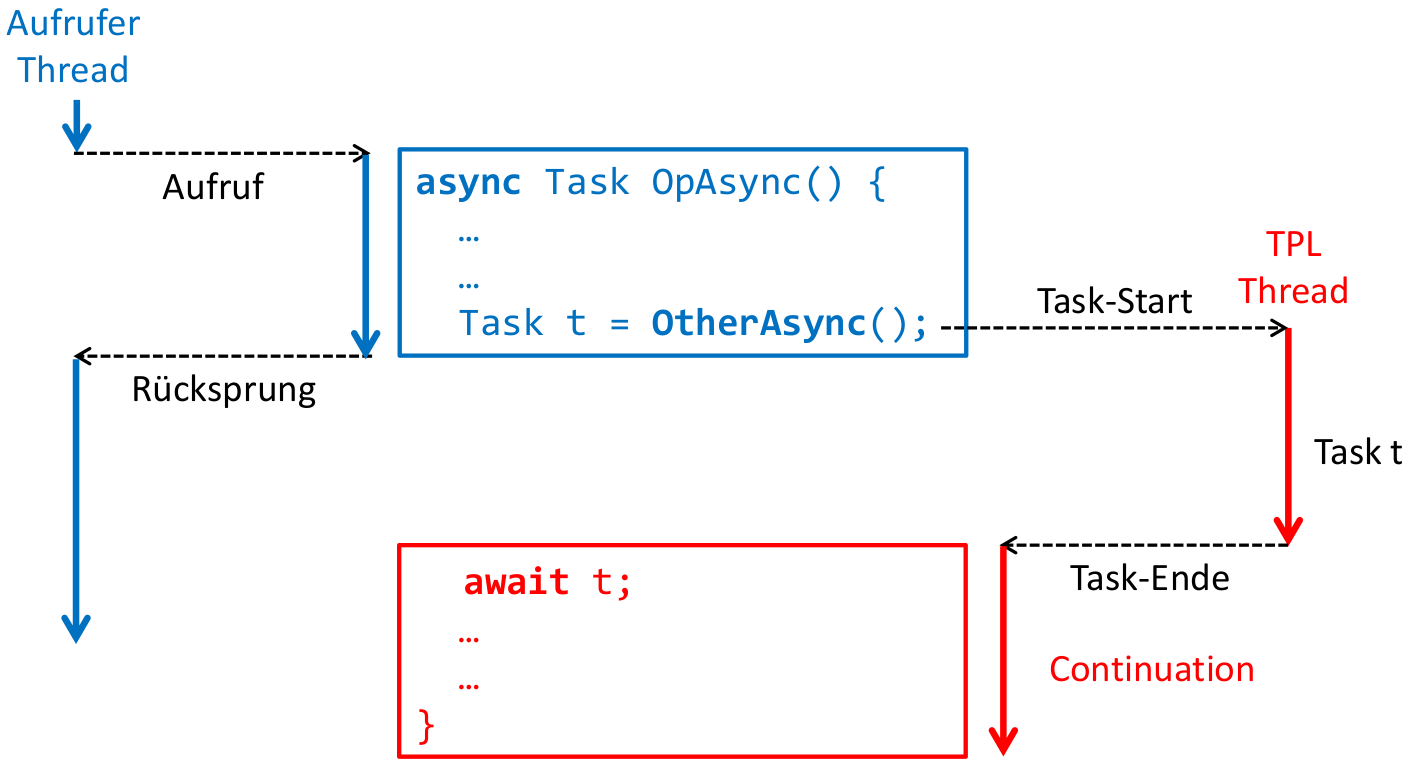
\includegraphics[width=0.7\linewidth]{03_ausfuehrung-thread.png}

Erster Abschnitt vor Await läuft Methode synchron durch Aufrufer, Abschnitt nach Await Läuft später nach Task-Ende (Continuation) in anderem Thread



\begin{lstlisting}
public async Task<int> LongOperationAsync() { ... }

Task<int> task = LongOperationAsync();
// Other Work
int result = await task; // Warte auf Beendigung der Async Methode, liefert Resultat des Tasks
\end{lstlisting}
